\documentclass{article}

% Language setting\usepackage[fontsize=12pt]{scrextend}
% Replace `english' with e.g. `spanish' to change the document language
\usepackage[french]{babel}
\usepackage{multicol}
\usepackage{multirow}
\usepackage{hhline}
% Set page size and margins
% Replace `letterpaper' with `a4paper' for UK/EU standard size
\usepackage[letterpaper,top=2cm,bottom=2cm,left=3cm,right=3cm,marginparwidth=1.75cm]{geometry}

% Useful packages
\usepackage[fontsize=12pt]{scrextend}
\usepackage{amsmath}
\usepackage{amsfonts}
\usepackage{graphicx}
\usepackage[colorlinks=true, allcolors=black]{hyperref}
\usepackage{textcomp}
\usepackage{eso-pic}
\usepackage{hyperref}
\usepackage{float}
\usepackage{fontspec}
\usepackage{todonotes}
%\usepackage{showframe}

\setlength{\parskip}{0.6\baselineskip}
\renewcommand{\baselinestretch}{1.1} 
\makeatletter
\renewcommand\paragraph{\@startsection{paragraph}{4}{\z@}%
            {-2.5ex\@plus -1ex \@minus -.25ex}%
            {1.25ex \@plus .25ex}%
            {\normalfont\normalsize\bfseries}}
\makeatother
\setcounter{secnumdepth}{4} % how many sectioning levels to assign numbers to
\setcounter{tocdepth}{4}    % how many sectioning levels to show in ToC
%\setlength{\baselineskip}{1\baselineskip}


\begin{document}


%%%%%% DEBUT PAGE DE GARDE %%%%%%%%%%%%%%%
\begin{titlepage}
    \begin{center}
        \textsc{\LARGE }\\[1.5cm]
        \vspace*{0.40cm}
        \textsc{\LARGE{NET 4103/7431 Homework \\
        Network science and Graph Learning}}\\
        \vspace*{0.40cm}
        \large{HOSTETTLER Maël\\}
        \href{mailto:mael.hostettler@telecom-sudparis.eu}{mael.hostettler@telecom-sudparis.eu}
        \vspace*{1cm}
        
        \textsc{\small{Projet de fin de module}}\\[1cm]
    \end{center}
    
    \vspace*{0.5cm}
    
    \begin{figure}[h]
        \begin{center}
            
\includegraphics[width=0.6\textwidth]{assets/logoTSP.png}
        \end{center}
    \end{figure}
    
    \vfill

    Télécom SudParis \hfill Année 2024/2025

\end{titlepage}

%%%%%% FIN COUVERTURE %%%%%%
\newpage
\tableofcontents
\newpage

\section{Introduction}

L'analyse de graphe est un sujet central à l'étude de plusieurs phénomènes, en particulier les communautés, les réseaux sociaux et les moteurs de recherche.
Grâce aux outils acquis lors du cours \texttt{NET 4103/7431} nous allons analyser le corpus de données Facebook100. Ce corpus de données décrit les liens d'amitié de différents élèves de 100 universités américaines.
L'échelle est donc significative, sans pour autant être tellement grande que l'on ne puisse conduire une telle analyse sur un ordinateur personnel.

L'analyse de ce corpus de données s'articule alors en 5 parties plutôt distinctes:

\begin{itemize}
    \item L'analyse des propriétés structurelles du graphe comme le clustering global/local
    \item L'analyse détaillée de l'assortativité par degré
    \item La prédiction de lien via trois métriques différentes
    \item La propagation d'étiquettes afin de retrouver/prédire certains attributs
    \item La détection ainsi que l'influence des concentrateurs de relations (hubs) à l'échelle locale est globale
\end{itemize}

Le code source de ce projet est disponible en ligne sur le dépôt suivant :~\url{https://github.com/maelhos/TSP-NET4103}.
Ce projet vise principalement à faire de l'analyse, donc à implémenter, exécuter et interpréter les résultats.
Cependant, dans la dernière partie, nous proposons un algorithme de détection de concentrateurs basé sur l'échantillonnage afin d'étudier la corrélation entre les concentrateurs et les individus avec beaucoup d'amis.

\section{Analyse structurelle}

\begin{tabular}{ |p{3.2cm}||p{3.2cm}|p{3.2cm}|p{3.2cm}|  }
    \hline
    \multicolumn{4}{|c|}{Coefficiant de regroupement} \\
    \hline
    Université & Global Clustering & Local Clustering & Edge density \\
    \hline
    Caltech & 0.29 & 0.41 & 0.06\\
    MIT& 0.18 & 0.27 & 0.01\\
    Johns Hopkins & 0.19 & 0.27 & 0.01\\
    \hline
\end{tabular}


On a ici deux cas de figures très flagrants: les étudiants de Caltech forment des communautés plus soudées, alors que MIT et Johns Hopkins forment un réseau moins connexe.
Il est important de noter que Caltech ont aussi un coefficient de clustering global plus élevé, ce qui pourrait indique que les communautés de Caltech ne sont pas plus soudées comme le laisserait penser le coefficient de clustering local et l'edge density, mais simplement plus nombreuses/denses.
Cependant, la différence de global clustering entre Caltech et les deux autres et bien plus faible que la différence de local clustering entre Caltech et les deux autres.
Il serait intéressant d'avoir une métrique qui analyse le clustering local indépendamment (au sens de la corrélation) du clustering global.


Dans les trois cas les graphes doivent être représenté de manière creuse, un ordre de grandeur donnée souvent dans la littérature (\textbf{"Graph Theory and Its Applications"} by \textsc{Jonathan Gross and Jay Yellen} par exemple) est:

\begin{itemize}
    \item $D < 0.1$: Représentation creuse
    \item $D > 0.5$: Représentation matricielle dense
    \item $0.1 \le D \le 0.5$: À voire, en fonction de l'application
\end{itemize}

Dans notre cas, comme la densité ne dépasse pas les $D = 0.06$, tout doit être représenté de manière creuse.
Une autre observation intéressante est la distribution des degrés. Celle-ci révèle qu'il y a exponentiellement moins d'individus avec de plus en plus d'amis.
Ce n'est pas étonnant, mais cela a un rôle important par la suite pour l'étude de concentrateurs (hubs).

\hfill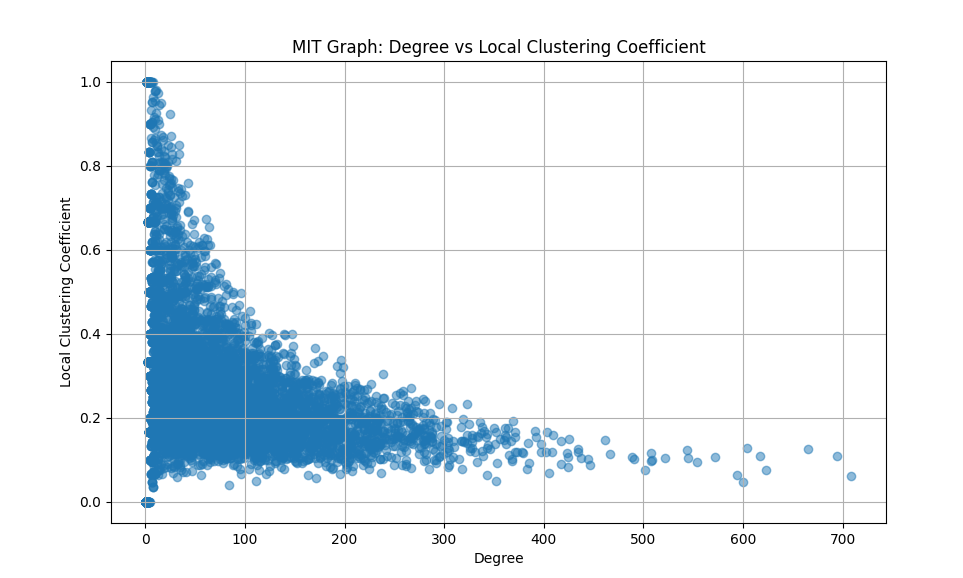
\includegraphics[width=0.5\textwidth]{assets/mit_clustering.png}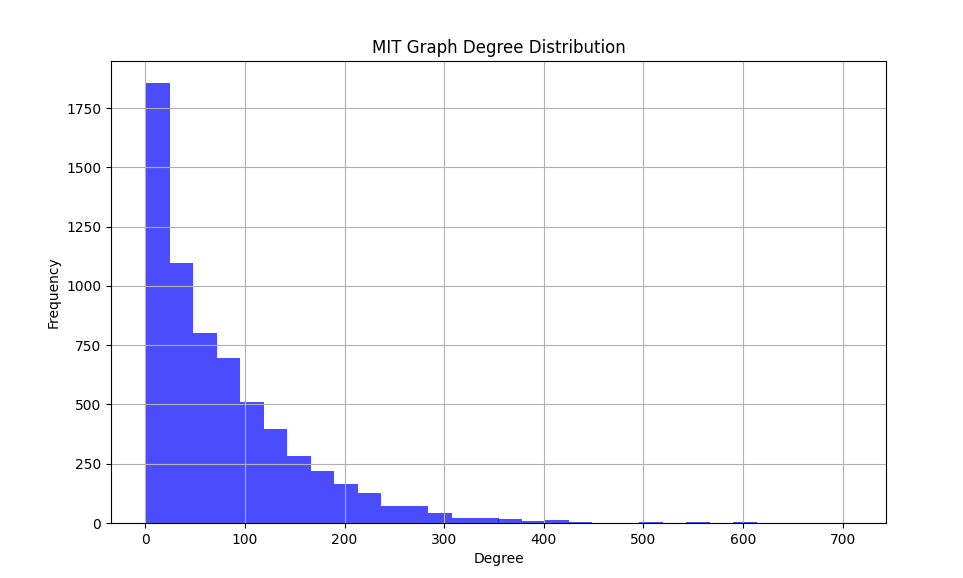
\includegraphics[width=0.5\textwidth]{assets/mit_deg_distrib.png}\hfill


\section{Analyse d'assortativité}

De manière générale, les individus ont une assortativité faible avec une concentration proche de $0$.
L'analyse d'assortativité nous mène une fois de plus vers les concentrateurs. En effet, on remarque que les différents liens d'amitiés ne sont pas très corrélés au nombre d'amis.
Autrement dit, quelqu'un qui a beaucoup d'amis a plutôt tendance à être ami avec des gens qui ont moins d'amis que lui.
Plus généralement, les nœuds avec des degrés proches ne sont pas particulièrement plus amis les uns avec les autres.

\hfill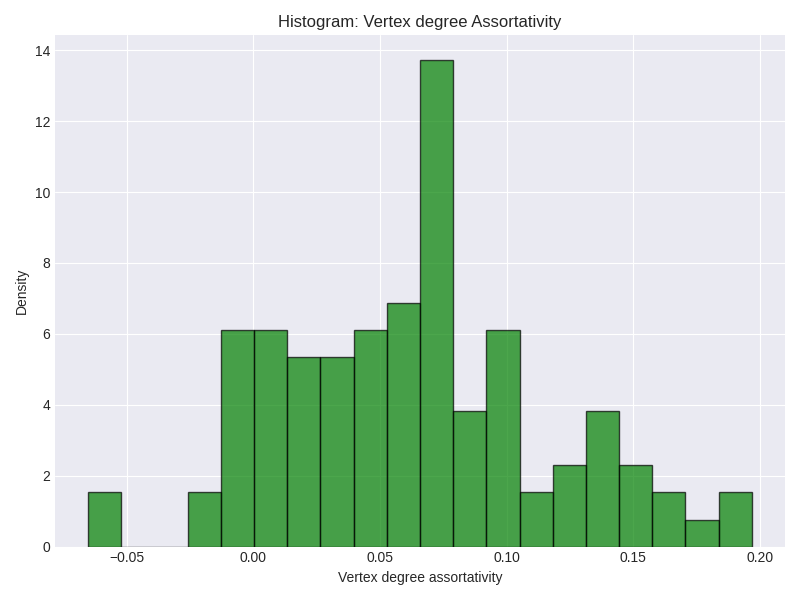
\includegraphics[width=0.8\textwidth]{assets/histogram_assortativity_degree.png}\hfill

L'assortativité n'est donc pas tant corrélée au degré, elle est plutôt corrélée aux attributs sociaux et personnels.

\section{Prédiction de lien}


Nous nous concentrerons sur le graph de Caltech afin de tester les trois métriques différents: Common Neighbors, Adamic-Adar, et Jaccard.

\begin{tabular}{ |p{4cm}||p{1cm}|p{3.2cm}|p{1.8cm}|p{1.1cm}|p{1.1cm}|  }
    \hline
    \multicolumn{6}{|c|}{Prédiction en fonction de la métriques choisie} \\
    \hline
    Métrique & k & Fraction enlevée & Précision & Recall & top-k \\
    \hline
    Common neighboor & 50  & 0.05 & 0.20 & 0.01 & 0.20 \\
                     & 50  & 0.2  & 0.38 & 0    & 0.38 \\
                     & 100 & 0.05 & 0.21 & 0.02 & 0.21 \\
                     & 100 & 0.2  & 0.41 & 0.01 & 0.41 \\
                     & 200 & 0.05 & 0.19 & 0.04 & 0.19 \\
                     & 200 & 0.2  & 0.38 & 0.02 & 0.38 \\
                     & 400 & 0.05 & 0.15 & 0.07 & 0.15 \\
                     & 400 & 0.2  & 0.36 & 0.04 & 0.36 \\
    \hhline{|=|=|=|=|=|=|}
    Adamic-Adar      & 50 & 0.05  & 0.28 & 0.02 & 0.28 \\
                     & 50 & 0.2   & 0.48 & 0.01 & 0.48 \\
                     & 100 & 0.05 & 0.24 & 0.03 & 0.24 \\
                     & 100 & 0.2  & 0.42 & 0.01 & 0.42 \\
                     & 200 & 0.05 & 0.20 & 0.05 & 0.20 \\
                     & 200 & 0.2  & 0.39 & 0.02 & 0.39 \\
                     & 400 & 0.05 & 0.17 & 0.08 & 0.17 \\
                     & 400 & 0.2  & 0.36 & 0.04 & 0.36 \\
    \hhline{|=|=|=|=|=|=|}
    Jaccard          & 50  & 0.05 & 0.14 & 0.01 & 0.14 \\
                     & 50  & 0.2  & 0.12 & 0.00 & 0.12 \\
                     & 100 & 0.05 & 0.11 & 0.01 & 0.11 \\
                     & 100 & 0.2  & 0.22 & 0.01 & 0.22 \\
                     & 200 & 0.05 & 0.13 & 0.03 & 0.13 \\
                     & 200 & 0.2  & 0.29 & 0.02 & 0.29 \\
                     & 400 & 0.05 & 0.11 & 0.05 & 0.11 \\
                     & 400 & 0.2  & 0.26 & 0.03 & 0.26 \\
    \hline
\end{tabular}

Pour la métrique Common neighboor, on remarque que celle-ci est assez sensible à la fraction de liens retirés plus qu'au nombre d'itérations. Cette métrique donne donc une meilleure information globale, mais est moins bonne quand on veut des informations précises sur quelques liens manquants.
En moyenne, Adamic-Ada est plus performante que Common neighboor avec des caractéristiques semblables à Common neighboor. Cette métrique est aussi moins sensible que Common neighboor.
Jaccard est intéressante, mais décevante. Cette métrique semble moins sensible à la proportion de liens enlevés, mais est trop peu performante pour être utile, et cela, peu importe le cas dans le cadre de cette étude.

Les métriquees Common Neighbors et Adamic-Adar sont plus efficaces et Adamic-Adar parait être la meilleure dans ce contexte. Cela n'est pas étonnant, car elle prend en compte la structure locale du réseau, ce qui est crucial dans le cas d'une étude de réseau social.


\section{Propagation d'étiquettes}

Nous allons désormais nous intéresser au problème de propagation d'étiquettes afin de retrouver des attributs manquants.
Tout les résultats seront sur le graph: MIT.

\begin{tabular}{ |p{2.5cm}||p{4cm}|p{2cm}|p{3cm}|  }
    \hline
    \multicolumn{4}{|c|}{Prédiction en fonction de la métriques choisie} \\
    \hline
    Attribut & Fraction enlevée & Précision & Erreur moyenne \\
    \hline
    Dorm             & 0.1 & 0.34 & 0.99 \\
                     & 0.2 & 0.32 & 1 \\
                     & 0.3 & 0.32 & 1 \\
    \hhline{|=|=|=|=|}
    Major index      & 0.1 & 0.24 & 5.35 \\
                     & 0.2 & 0.21 & 5.14 \\
                     & 0.3 & 0.21 & 5.49 \\
    \hhline{|=|=|=|=|}
    Gender           & 0.1 & 0.55 & 0.54 \\
                     & 0.2 & 0.53 & 0.56 \\
                     & 0.3 & 0.53 & 0.55 \\
    \hline
\end{tabular}

On remarque que les attributs "Dorm" et "Gender" sont bien mieux retrouvés que "Major index".
Cela n'est pas très étonnant non plus, car notre score ne prend pas en compte le biais d'erreur.
Il n'y a qu'une chance sur deux de se tromper sur le genre (enfin... presque...) alors qu'il n'y a qu'un seul "Major index" juste parmi une liste non binaire.
Il faudrait donc une métrique plus adaptée afin de comparer plus justement.

\section{Concentrateurs}

Nous nous intéressons ici aux concentrateurs ou hubs en anglais. Il s'agit grossièrement des individus avec beaucoup d'amis, même si cette définition n'est pas forcément la plus intéressante.
Ce qui nous intéresse, ce n'est pas juste les individus avec beaucoup d'amis, ce sont plutôt ceux qui participent fortement à la connectivité globale.
Dans le cadre d'un réseau social à l'échelle d'un campus, ce phénomène est peut-être moins prépondérant qu'en pratique (avec les célébrités et les personnalités politiques), mais cette étude reste tout de même intéressante.

L'hypothèse que l'on émet est que dans le cadre de ce dataset, les hubs risquent d'être les individus avec le plus d'amis, même si dans la réalité, sur Facebook complet, potentiellement pas.
Dans un premier temps, nous allons proposer un algorithme afin de calculer le top $n\textrm{--}\texttt{HUB}$.
C'est-à-dire les $n$ individus les plus importants pour la connectivité globale. Comme il est trivial de calculer les $n$ individus avec le plus d'amis, on pourra par la suite s'intéresser à la taille de l'intersection de ces deux ensembles proportionnellement à $n$.

Comme en pratique, on aura des représentations creuses sur des graphes très grands, on ne peut utiliser les puissances de la matrice d'adjacence.
Nous proposons une méthode Monte-Carlo basée sur l'échantillonnage.

Soit un graph $G = (V, E)$, et deux paramètres $(k, n) \in \mathbb N^2, n \le |V|$:

\begin{itemize}
    \item On initialise un tableau de taille $|V|$ rempli de $0$
    \item Répéter $k$ fois:
    \begin{itemize}
        \item Choisir $(n_1, n_2) \in V^2$ aléatoirement
        \item En utilisant l'algorithme de Dijkstra pour calculer les chemins les plus courts entre $n_1$ et $n_2$
        \item Incrémenter le score dans le tableau de chaque nœud sur le chemin appart $n_1$ et $n_2$ pour chaque occurrence sur les chemins les plus courts
    \end{itemize}
    \item Retourner les $n$ premiers hubs au sens de ce score
\end{itemize}

Cet algorithme a une complexité de: $\mathcal O(k(|E| + |V| \log(|V|)))$, la convergence théorique de cet algorithme en théorie n'est probablement pas évidente, mais les résultats expérimentaux tendent à montrer que l'algorithme convergent.
Nous avons fait le choix de considérer le cas général où il existe plusieurs plus courts chemins. Il faut donc gérer ce cas.
Aussi, nous avons choisi le plus court chemin, car il représente bien quelqu'un de social et polyvalent qui n'est pas juste membre d'une communauté très connexe.
L'idée de plus court chemin est de "pénaliser" le fait d'être dans une communauté très connexe, car dans ce cas, les plus courts chemins ont moins de chance de passer par un individu, même s'il a beaucoup d'amis.
On pourrait aussi considérer tous les chemins en utilisant Floyd-Warshall mais la complexité monte en $\mathcal O(|V|^3)$


\begin{tabular}{ |p{3.5cm}||p{1cm}|p{2cm}|p{3cm}|  }
    \hline
    \multicolumn{4}{|c|}{Corrélation top-amis vs top-hub} \\
    \hline
    Réseau & k & top-n & Corrélation \\
    \hline
    Caltech          & 200  & 10 & 0.5 \\
                     & 800  & 10 & 0.7 \\
                     & 1600 & 10 & 0.6 \\
                     & 200  & 100 & 0.7 \\
                     & 800  & 100 & 0.78 \\
                     & 1600 & 100 & 0.8 \\
                     & 200  & 1000 & 0.77 \\
                     & 800  & 1000 & 0.77 \\
                     & 1600 & 1000 & 0.77 \\
    \hhline{|=|=|=|=|}
    MIT              & 200  & 10 & 0.4 \\
                     & 800  & 10 & 0.5 \\
                     & 1600 & 10 & 0.6 \\
                     & 200  & 100 & 0.44 \\
                     & 800  & 100 & 0.63 \\
                     & 1600 & 100 & 0.61 \\
                     & 200  & 1000 & 0.61 \\
                     & 800  & 1000 & 0.72 \\
                     & 1600 & 1000 & 0.76 \\
    \hhline{|=|=|=|=|}
    Johns Hopkins    & 200  & 10 & 0.2 \\
                     & 800  & 10 & 0.3 \\
                     & 1600 & 10 & 0.4 \\
                     & 200  & 100 & 0.41 \\
                     & 800  & 100 & 0.51 \\
                     & 1600 & 100 & 0.54 \\
                     & 200  & 1000 & 0.64 \\
                     & 800  & 1000 & 0.74 \\
                     & 1600 & 1000 & 0.77 \\
    \hline
\end{tabular}

Selon le graphe, on remarque que la convergence est plus ou moins rapide, par exemple pour Caltech celle-ci est très rapide.
Alors que pour MIT Johns Hopkins elle est un peu plus lente.

Nous allons nous concentrer sur les valeurs de $k$ les plus grandes (donc $k = 1600$), car elles sont les plus représentatives. Les valeurs de $k$ plus basses sont la juste pour étudier la convergence.
On remarque que pour $n = 1000$ les trois réseaux ont le même comportement. Il s'agit là d'un comportement limite, on a pris "trop" d'éléments du top avec le plus d'amis et on n'a donc plus vraiment des hubs.

La donnée la plus intéressante est pour $n = 100$, on a alors $0.8$ pour Caltech, $0.61$ pour MIT et $0.54$ pour Johns Hopkins. Les valeurs plus proches de $1$ signifient que les concentrateurs sont les individus avec le plus d'amis et les valeurs plus proches de $0$ l'inverse.
Une manière de l'interpréter: la corrélation est plus faible, donc c'est que des individus avec moins d'amis font plus de goulots d'étranglement entre différentes composantes connexes.
Une conclusion possible est que les valeurs plus proches de $0$ indiquent alors une école plus cosmopolite et avec des communautés plus ouvertes.


\end{document}